

\tikzset{every picture/.style={line width=0.75pt}} %set default line width to 0.75pt        

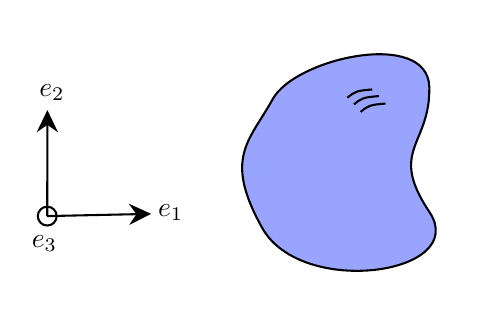
\begin{tikzpicture}[x=0.75pt,y=0.75pt,yscale=-1,xscale=1]
%uncomment if require: \path (0,147); %set diagram left start at 0, and has height of 147

%Straight Lines [id:da714513522153384] 
\draw    (204.92,106.08) -- (205,58) ;
\draw [shift={(205,55)}, rotate = 450.09] [fill={rgb, 255:red, 0; green, 0; blue, 0 }  ][line width=0.08]  [draw opacity=0] (10.72,-5.15) -- (0,0) -- (10.72,5.15) -- (7.12,0) -- cycle    ;
%Straight Lines [id:da5515121753638923] 
\draw    (204.92,106.08) -- (252,105.06) ;
\draw [shift={(255,105)}, rotate = 538.76] [fill={rgb, 255:red, 0; green, 0; blue, 0 }  ][line width=0.08]  [draw opacity=0] (10.72,-5.15) -- (0,0) -- (10.72,5.15) -- (7.12,0) -- cycle    ;
%Shape: Polygon Curved [id:ds9724076255877165] 
\draw  [fill={rgb, 255:red, 0; green, 27; blue, 255 }  ,fill opacity=0.4 ] (313.5,49.8) .. controls (324.5,29.8) and (388.5,15.8) .. (389,44) .. controls (389.5,72.2) and (369,74) .. (389,104) .. controls (409,134) and (327.5,145.8) .. (308.5,111.8) .. controls (289.5,77.8) and (302.5,69.8) .. (313.5,49.8) -- cycle ;
%Curve Lines [id:da4789715178338929] 
\draw    (352.7,52.27) .. controls (356.37,49.27) and (357.1,48.84) .. (364.7,48.27) ;
%Curve Lines [id:da4708439042769508] 
\draw    (355.9,55.87) .. controls (359.57,52.87) and (360.3,52.44) .. (367.9,51.87) ;
%Curve Lines [id:da6677145112477441] 
\draw    (349.5,49.07) .. controls (353.17,46.07) and (353.9,45.64) .. (361.5,45.07) ;
%Shape: Circle [id:dp04858550264997041] 
\draw   (200.38,106.08) .. controls (200.38,103.57) and (202.41,101.54) .. (204.92,101.54) .. controls (207.43,101.54) and (209.46,103.57) .. (209.46,106.08) .. controls (209.46,108.59) and (207.43,110.62) .. (204.92,110.62) .. controls (202.41,110.62) and (200.38,108.59) .. (200.38,106.08) -- cycle ;

% Text Node
\draw (256.8,99.1) node [anchor=north west][inner sep=0.75pt]    {$\vt{e}_{1}$};
% Text Node
\draw (199.6,41.2) node [anchor=north west][inner sep=0.75pt]    {$\vt{e}_{2}$};
% Text Node
\draw (196,113.8) node [anchor=north west][inner sep=0.75pt]    {$\vt{e}_{3}$};


\end{tikzpicture}
